\subsection*{Insecure Direct Object Reference -- Unauthorized Basket Access (IDOR)}

\begin{table}[H]
\centering
\begin{tabular}{|l|p{10cm}|}
\hline
\textbf{Finding ID} & IDOR \\
\hline
\textbf{Severity} & Medium \\
\hline
\textbf{CVSS 3.1 Score} & 6.5 (Medium) \\
\hline
\textbf{CVSS Vector} & \texttt{AV:N/AC:L/PR:L/UI:N/S:U/C:H/I:N/A:N} \\
\hline
\textbf{Status} & Confirmed \\
\hline
\textbf{OWASP Category} & A01:2021 -- Broken Access Control \\
\hline
\textbf{CWE} & CWE-639 -- Authorization Bypass Through User-Controlled Key \\
\hline
\textbf{Affected Endpoint} & \verb|GET /rest/basket/{id}| \\
\hline
\textbf{Affected Parameter} & \texttt{id} (basket ID in URL path) \\
\hline
\end{tabular}
\caption{Insecure Direct Object Reference finding details}
\end{table}

\subsubsection*{Description}

The basket endpoint uses the basket ID provided in the URL to return
basket information. However, the application does not properly check
whether the requested basket belongs to the logged-in user.

During testing, the basket ID was changed from one value to another
while using the same authenticated session. The application returned
basket information for a different user instead of denying access.

This is an Insecure Direct Object Reference (IDOR) vulnerability. It
occurs when an application uses a user-controlled object identifier
without properly verifying whether the authenticated user is
authorized to access that object.

\subsubsection*{Methodology}

The basket functionality was tested using Burp Suite. A normal basket
request was first captured and the basket ID in the URL was identified.
The ID was then changed to another value while keeping the same
authenticated session.

The response was examined to determine whether the application
properly verified ownership of the requested basket.

\subsubsection*{Steps to Reproduce}

\begin{enumerate}

    \item Log in as a normal user and open the shopping basket.

    \item Capture the basket request using Burp Suite.

    \item Observe the basket ID in the request, for example:

    \begin{lstlisting}
GET /rest/basket/7
    \end{lstlisting}

    \item Send the request and confirm that the application returns
    the basket associated with the current user.

    \item Change the basket ID to another value, for example:

    \begin{lstlisting}
GET /rest/basket/5
    \end{lstlisting}

    \item Send the modified request using the same authenticated
    session.

    \item Observe that the application returns the contents of another
    basket instead of returning an access-denied response.

\end{enumerate}

\subsubsection*{Evidence}

\begin{figure}[H]
    \centering
    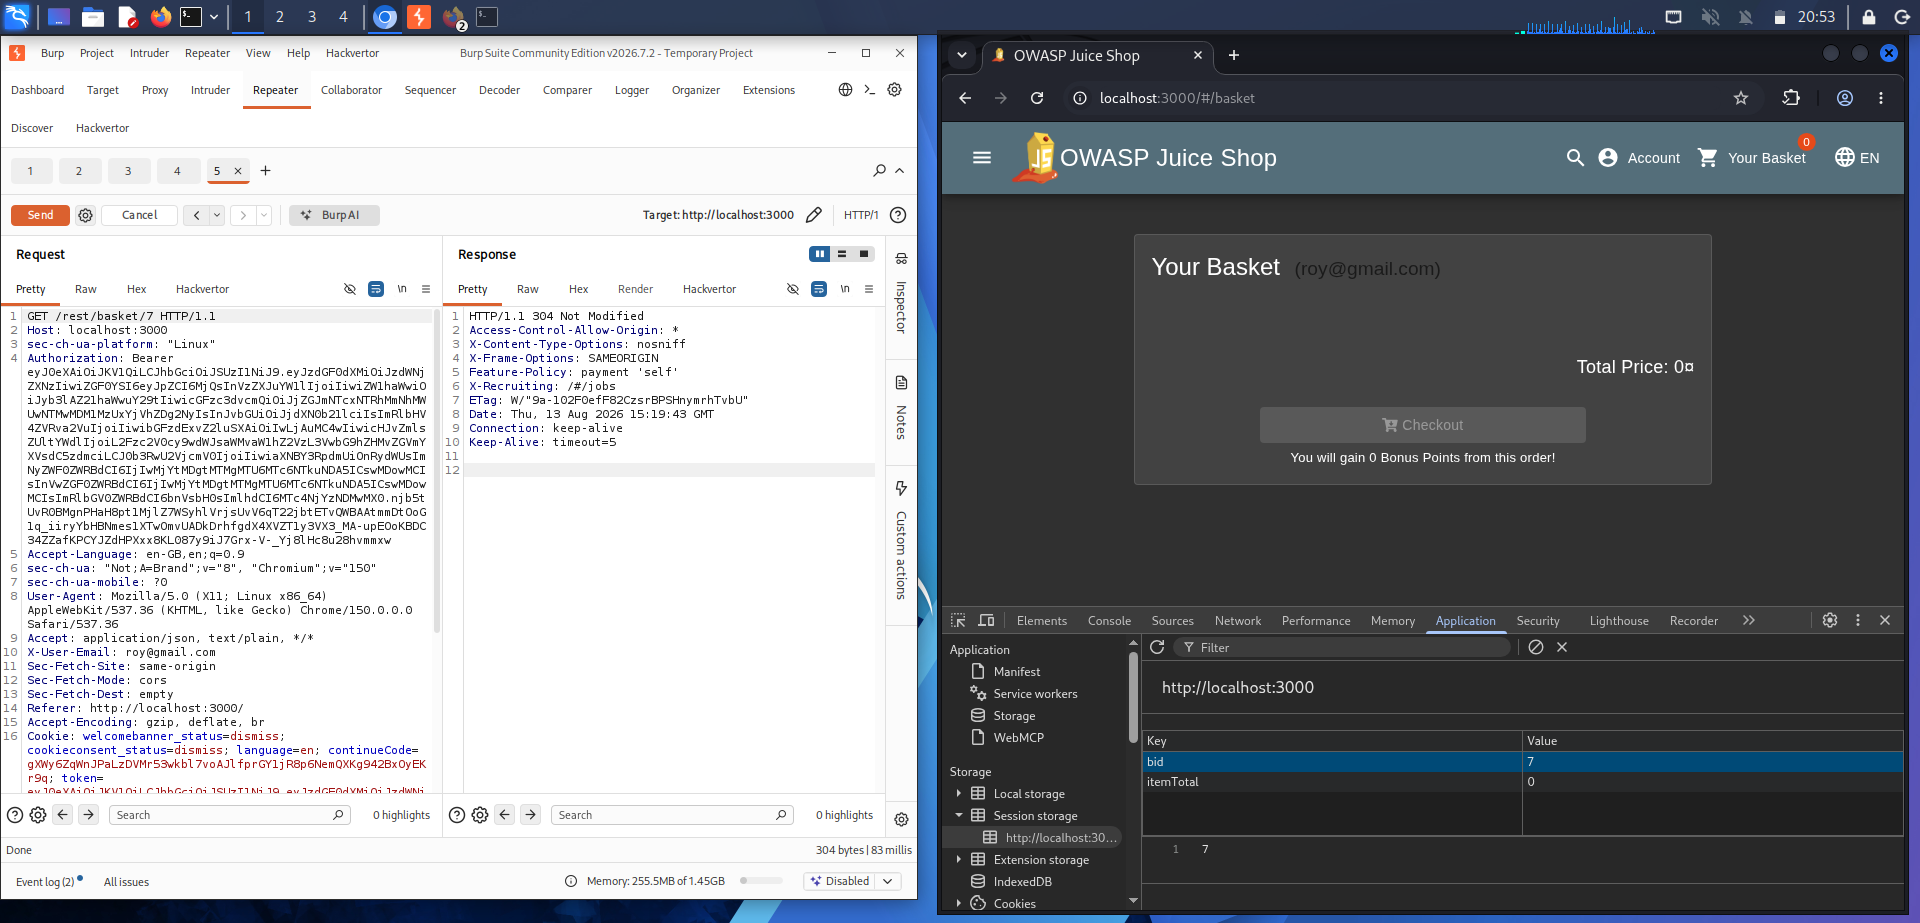
\includegraphics[width=0.8\textwidth]
    {evidence/phase4/idor/idor01-01-original-basket-request.png}
    \caption{Original basket request using the basket ID associated with the logged-in user}
\end{figure}

\begin{figure}[H]
    \centering
    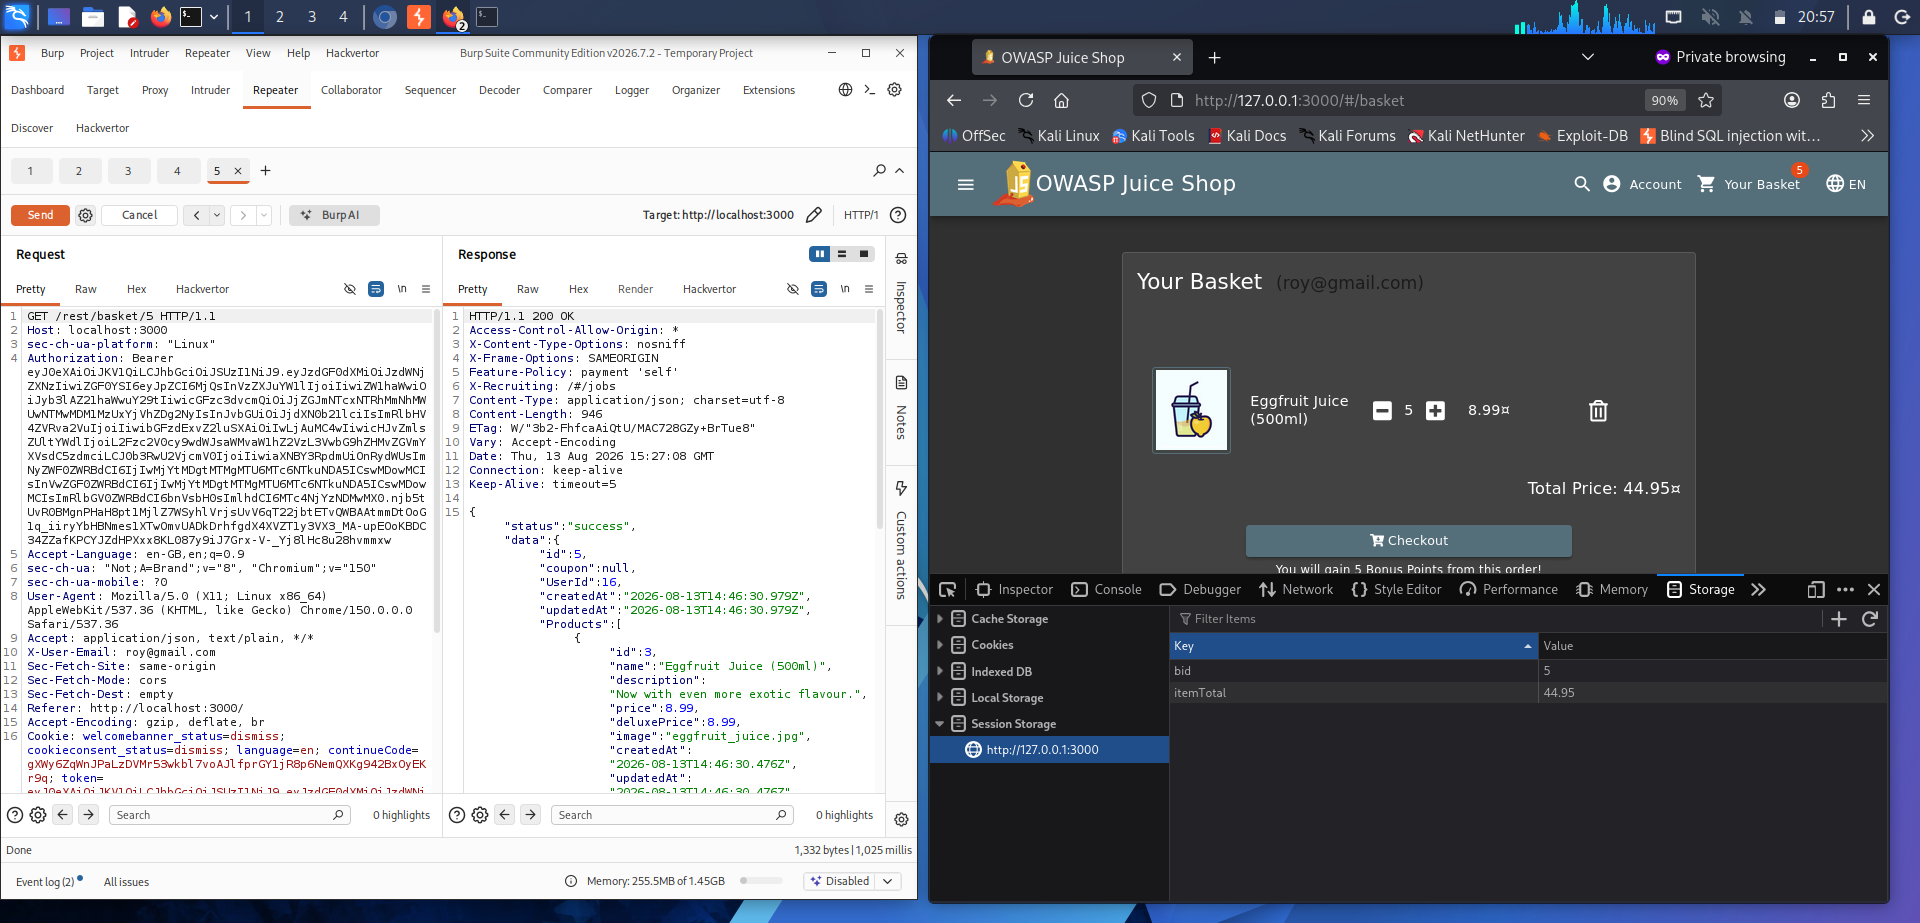
\includegraphics[width=0.8\textwidth]
    {evidence/phase4/idor/idor01-02-unauthorized-basket-access.png}
    \caption{Modified basket ID returning another user's basket data}
\end{figure}

\subsubsection*{Impact}

A logged-in user can access another user's basket by changing the
basket ID in the request.

This can expose information about another user's shopping activity,
including the products and quantities stored in the basket.

If basket identifiers are predictable, an attacker may also be able
to test additional identifiers and access other baskets when the same
authorization weakness exists.

\subsubsection*{Remediation}

\begin{itemize}

    \item Verify on the server side that the requested basket belongs
    to the currently authenticated user.

    \item Deny access when the user does not have permission to access
    the requested basket.

    \item Do not rely solely on the basket ID supplied by the client
    to determine authorization.

    \item Apply the same server-side ownership checks to other
    user-specific resources such as orders, profiles, and payment
    information.

    \item Use unpredictable object identifiers where appropriate as
    an additional security measure. This must not replace proper
    authorization checks.

\end{itemize}

\subsubsection*{Conclusion}

The IDOR vulnerability was successfully confirmed by modifying the
basket ID in an authenticated request.

The application returned another user's basket data without verifying
whether the logged-in user was authorized to access the requested
basket.

The finding is therefore classified as a confirmed Medium-severity
Broken Access Control vulnerability.